\documentclass[11pt]{article}

%% PACKAGES
\usepackage{graphicx}
\usepackage[printonlyused]{acronym}
\usepackage{float}
\usepackage[colorlinks=false]{hyperref}
\usepackage{caption}
\usepackage{tabularx}
\usepackage[margin=1.0in]{geometry}
\usepackage{tocloft}

\makeatletter
\g@addto@macro\normalsize{%
  \setlength\abovedisplayskip{0.25pt}
  \setlength\belowdisplayskip{0.25pt}
  \setlength\abovedisplayshortskip{0.25pt}
  \setlength\belowdisplayshortskip{0.25pt}
}
\makeatother

\setlength{\parskip}{\baselineskip}

%% GRAPHICS PATH
\graphicspath{{../../../shared_latex_inputs/images}{../../../shared_latex_inputs/graphs}}

\newcommand{\acposs}[1]{%
	\expandafter\ifx\csname AC@#1\endcsname\AC@used
	\acs{#1}'s%
	\else
	\aclu{#1}'s (\acs{#1}'s)%
	\fi
}

\title{\Huge EMTG Tutorial: OSIRIS-REx}
\vspace{0.5cm}
\author
{
	Tim Sullivan \thanks{Aerospace Engineer, The Aerospace Corporation}
}
\vspace{0.5cm}

\newcommand{\listofknownissuesname}{\Large List of Known Issues}
\newlistof{knownissues}{mcf}{\listofknownissuesname}

\newcommand{\knownissue}[3]
{
	\refstepcounter{knownissues}
	\par\noindent\textbf{\hyperref[#2_b]{\theknownissues\quad #1}}\label{#2_h}
	\textbf{\hfill\pageref{#2_b}}
	#3
}

\newcommand{\knownissuelabel}[2]
{
	 \phantomsection
  	\hyperref[#2_h]{#1}\def\@currentlabel{\unexpanded{#1}}\label{#2_b}
}

\begin{document}

\begin{titlepage}
\maketitle
\thispagestyle{empty}
\begin{table}[H]
	\centering
	\begin{tabularx}{\textwidth}{|l|l|X|}
		\hline
		\textbf{Revision Date} & \textbf{Author} & \textbf{Description of Change} \\
		\hline
		\date{December 2, 2022} & Tim Sullivan & Initial revision.\\
		\hline
		\date{June 30, 2023} & Joseph Hauerstein & Conversion to \LaTeX.\\ 
		\hline
		\date{August 4, 2023} & Joseph Hauerstein & Addition of Known Issues section.\\ 
		\hline
	\end{tabularx}
\end{table}
\end{titlepage}

\newpage
\tableofcontents
\thispagestyle{empty}
\newpage

\listofknownissues
\thispagestyle{empty}

\knownissue{Bug opening EMTG options file in text editor using PyEMTG}{text_editor_issue}

\newpage
\clearpage
\setcounter{page}{1}



\section*{List of Acronyms}
\begin{acronym}
%To define the acronym and include it in the list of acronyms: \acro{acronym}{definition}
%To define the acronym and exclude it from the list of acronyms:  \acro{acronym}{definition}
%
%\ac{acronym} Expand and identify the acronym the first time; use only the acronym thereafter
%\acf{acronym} Use the full name of the acronym.
%\{acronym} Use the acronym, even before the first corresponding \ac command
%\acl{acronym}  Expand the acronym without using the acronym itself.
%
%

\acro{ACS}{attitude control system}
\acro{ACO}{Ant Colony Optimization}
\acro{AD}{Automatic Differentiation}
\acro{ADL}{Architecture Design Laboratory}
\acro{AES}{Advanced Exploration Systems}
\acro{AGA}{aerogravity assist}
\acro{ALARA}{As Low As Reasonably Achievable}
\acro{API}{application programming interface}
\acro{BB}{branch and bound}
\acro{BVP}{Boundary Value Problem}
\acro{CATO}{Computer Algorithm for Trajectory Optimization}
\acro{CL}{confidence level}
\acro{CONOPS}{concept of operations}
\acro{COV}{Calculus of Variations}
\acro{D/AV}{Descent/Ascent Vehicle}
\acro{DE}{Differential Evolution}
\acro{DLA}{Declination of Launch Asymptote}
\acro{RLA}{Right Ascension of Launch Asymptote}
\acro{RA}{right ascension}
\acro{DEC}{declination}
\acro{DPTRAJ/ODP}{Double Precision Trajectory and Orbit Determination Program}
\acro{DSH}{Deep Space Habitat}
\acro{DSN}{Deep Space Network}
\acro{DSMPGA}{Dynamic-Size Multiple Population Genetic Algorithm}
\acro{EB}{Evolutionary Branching}
\acro{ECLSS}{environmental control and life support system}
\acro{ELV}{expendable launch vehicle}
\acro{EMME}{Earth to Mars, Mars to Earth}
\acro{EMMVE}{Earth to Mars, Mars to Venus to Earth}
\acro{EMTG}{Evolutionary Mission Trajectory Generator}
\acro{EVMME}{Earth to Venus to Mars, Mars to Earth}
\acro{EVMMVE}{Earth to Venus to Mars, Mars to Venus to Earth}
\acro{ERRV}{Earth Return Re-entry Vehicle}
\acro{FISO}{Future In-Space Operations}
\acro{FMT}{Fast Mars Transfer}
\acro{GASP}{Gravity Assist Space Pruning}
\acro{GCR}{galactic cosmic radiation}
\acro{GRASP}{Greedy Randomized Adaptive Search Procedure}
\acro{GSFC}{Goddard Space Flight Center}
\acro{GTOC}{Global Trajectory Optimization Competition}
\acro{GTOP}{Global Trajectory Optimization Problem}
\acro{HAT}{Human Architecture Team}
\acro{HGGA}{Hidden Genes Genetic Algorithm}
\acro{IMLEO}{Initial Mass in \acl{LEO}}
\acro{IPOPT}{Interior Point OPTimizer}
\acro{ISS}{International Space Station}
\acro{JHUAPL}{Johns Hopkins University Applied Physics Laboratory}
\acro{JSC}{Johnson Space Center}
\acro{KKT}{Karush-Kuhn-Tucker}
\acro{LEO}{Low Earth Orbit}
\acro{LRTS}{lazy race tree search}
\acro{MONTE}{Mission analysis, Operations, and Navigation Toolkit Environment}
\acro{MCTS}{Monte Carlo tree search}
\acro{MGA}{Multiple Gravity Assist}
\acro{MIRAGE}{Multiple Interferometric Ranging Analysis using GPS Ensemble}
\acro{MOGA}{Multi-Objective Genetic Algorithm}
\acro{MOSES}{Multiple Orbit Satellite Encounter Software}
\acro{MPI}{message passing interface}
\acro{MPLM}{Multi-Purpose Logistics Module}
\acro{MSFC}{Marshall Space Flight Center}
\acro{NELLS}{NASA Exhaustive Lambert Lattice Search}
\acro{NSGA}{Non-Dominated Sorting Genetic Algorithm}
\acro{NSGA-II}{Non-Dominated Sorting Genetic Algorithm II}
\acro{NHATS}{Near-Earth Object Human Space Flight Accessible Targets Study}
\acro{NTP}{Nuclear Thermal Propulsion}
\acro{OD}{orbit determination}
\acro{OOS}{On-Orbit Staging}
\acro{PCC}{Pork Chop Contour}
\acro{PEL}{permissible exposure limits}
\acro{PLATO}{PLAnetary Trajectory Optimization}
\acro{REID}{risk of exposure-induced death}
\acro{RTBP}{Restricted Three Body Problem}
\acro{SA}{Simulated Annealing}
\acro{SLS}{Space Launch System}
\acro{SNOPT}{Sparse Nonlinear OPTimizer}
\acro{SOI}{sphere of influence}
\acro{SPE}{solar particle events}
\acro{SQP}{sequential quadratic programming}
\acro{SRAG}{Space Radiation Analysis Group}
\acro{TEI}{Trans-Earth Injection}
\acro{TOF}{time of flight}
\acro{TPBVP}{Two Point Boundary Value Problem}
\acro{TMI}{Trans-Mars Injection}
\acro{VARITOP}{Variational calculus Trajectory Optimization Program}
\acro{VILM}{v-infinity leveraging maneuver}
\acro{MOI}{Mar Orbit Injection}
\acro{PCM}{Pressurized Cargo Module}
\acro{STS}{Space Transportation System}
\acro{EDS}{Earth Departure Stage}
\acro{NEO}{near-Earth asteroid}
\acro{IDC}{Integrated Design Center}
\acro{SEP}{solar-electric propulsion}
\acro{SRP}{solar radiation pressure}
\acro{NEP}{nuclear-electric propulsion}
\acro{REP}{radioisotope-electric propulsion}
\acro{DRM}{Design Reference Missions}

\acro{EDL}{entry, descent, and landing}
\acro{ASCII}{American Standard Code for Information Interchange}
\acro{AU}{Astronomical Unit}
\acro{BWG}{Beam Waveguides}
\acro{CCB}{Configuration Control Board}
\acro{CMO}{Configuration Management Office}
\acro{CODATA}{Committee on Data for Science and Technology}
\acro{DEEVE}{Dynamically Equivalent Equal Volume Ellipsoid}
\acro{DRA}{Design Reference Asteroid}
\acro{EME2000}{Earth Centered, Earth Mean Equator and Equinox of J2000 (Coordinate Frame)}
\acro{EOP}{Earth Orientation Parameters}
\acro{ET}{Ephemeris Time}
\acro{FDS}{Flight Dynamics System}
\acro{FTP}{File Transfer Protocol}
\acro{GSFC}{Goddard Space Flight Center}
\acro{PI}{Principal Investigator}
\acro{HEF}{High Efficiency}
\acro{IAG}{International Association of Geodesy}
\acro{IAU}{International Astronomical Union}
\acro{IERS}{International Earth Rotation and Reference Systems Service}
\acro{ICRF}{International Celestial Reference Frame}
\acro{ITRF}{International Terrestrial Reference System}
\acro{IOM}{Interoffice Memorandum}
\acro{JD}{Julian Date}
\acro{JPL}{Jet Propulsion Laboratory}
\acro{LM}{Lockheed Martin}
%\acro{LP150Q}{}
%\acros{LP100K}{}
\acro{MAVEN}{Mars Atmosphere and Volatile EvolutioN}
\acro{MJD}{Modified Julian Date}
\acro{MOID}{Minimum Orbit Intersection Distance}
\acro{MPC}{Minor Planet Center}
\acro{NASA}{National Aeronautics and Space Administration}
\acro{NDOSL}{\ac{NASA} Directory of Station Locations}
\acro{NEA}{near-Earth asteroid}
\acro{NEO}{near-Earth object}
\acro{NIO}{Nav IO}
\acro{OSIRIS-REx}{Origins Spectral Interpretation Resource Identification Security-Regolith Explorer}
\acro{PHA}{Potentially Hazardous Asteroid}
\acro{PHO}{Potentially Hazardous Object}
\acro{SBDB}{Small-Body Database}
\acro{SI}{International System of Units}
\acro{SPICE}{Spacecraft Planet Instrument Camera-matrix Events}
\acro{SPK}{SPICE Kernel}
\acro{SRC}{Sample Return Capsule}
\acro{SSD}{Solar System Dynamics}
\acro{STK}{Systems Tool Kit}
\acro{TAI}{International Atomic Time}
\acro{TBD}{To Be Determined}
\acro{TBR}{To Be Reviewed}
\acro{TCB}{Barycentric Coordinate Time}
\acro{TDB}{Temps Dynamiques Barycentrique, Barycentric Dynamical Time}
\acro{TDT}{Terrestrial Dynamical Time}
\acro{TT}{Terrestrial Time}
\acro{URL}{Uniform Resource Locator}
\acro{UT}{Universal Time}
\acro{UT1}{Universal Time Corrected for Polar Motion}
\acro{UTC}{Coordinated Universal Time}
\acro{USNO}{U. S. Naval Observatory}
\acro{YORP}{Yarkovsky-O'Keefe-Radzievskii-Paddack}

\acro{NLP}{nonlinear program}
\acro{MBH}{monotonic basin hopping}
\acro{MBH-C}{monotonic basin hopping with Cauchy hops}
\acro{FBS}{forward-backward shooting}
\acro{MGALT}{Multiple Gravity Assist with Low-Thrust}
\acro{MGALTS}{Multiple Gravity Assist with Low-Thrust using the Sundman transformation}
\acro{MGA-1DSM}{Multiple Gravity Assist with One Deep Space Maneuver}
\acro{MGAnDSMs}{Multiple Gravity Assist with \textit{n} Deep-Space Maneuvers using Shooting}
\acro{PSFB}{Parallel Shooting with Finite-Burn}
\acro{PSBI}{Parallel Shooting with Bounded Impulses}
\acro{FBLT}{Finite-Burn Low-Thrust}
\acro{FBLTS}{Finite-Burn Low-Thrust using the Sundman transformation}
\acro{ESA}{European Space Agency}
\acro{ACT}{Advanced Concepts Team}
\acro{IRAD}{independent research and development}
\acro{Isp}[$\text{I}_{sp}$]{specific impulse}
\acro{C3}[$C_3$]{hyperbolic excess energy}
\acro{GA}{genetic algorithm}
\acro{GALLOP}{ Gravity Assisted Low-thrust Local Optimization Program}
\acro{MALTO}{Mission Analysis Low-Thrust Optimization}
\acro{PaGMO}{Parallel Global Multiobjective Optimizer}
\acro{FRA}{feasible region analysis}
\acro{CP}{conditional penalty}
\acro{HOC}{hybrid optimal control}
\acro{HOCP}{hybrid optimal control problem}
\acro{PSO}{particle swarm optimization}
\acro{SEPTOP}{Solar Electric Propulsion Trajectory Optimization Program}
\acro{STOUR}{Satellite Tour Design Program}
\acro{STOUR-LTGA}{Satellite Tour Design Program - Low Thrust, Gravity Assist}
\acro{PaGMO}{Parallel Global Multiobjective Optimizer}
\acro{SDC}{static/dynamic control}
\acro{DDP}{Differential Dynamic Programming}
\acro{HDDP}{Hybrid Differential Dynamic Programming}
\acro{ACT}{Advanced Concepts Team}
\acro{GMAT}{General Mission Analysis Toolkit}
\acro{BOL}{beginning of life}
\acro{EOL}{end of life}
\acro{KSC}{Kennedy Space Center}
\acro{VSI}{variable \ac{Isp}}
\acro{RTG}{radioisotope thermal generator}
\acro{ASRG}{advanced Stirling radiosotope generator}
\acro{ARRM}{Asteroid Robotic Redirect Mission}
\acro{AATS}{Alternative Architecture Trade Study}
\acro{PPU}{power processing unit}
\acro{STM}{state transition matrix}
\acro{MTM}{maneuver transition matrix}
\acro{HPTM}{half-phase transition matrix}
\acro{BCI}{body-centered inertial}
\acro{BCF}{body-centered fixed}
\acro{UTTR}{Utah Test and Training Range}
\acro{EPV}{equatorial projection of $\mathbf{v}_\infty$}
\acro{KBO}{Kuiper belt object}
\acro{DSM}{deep-space maneuver}
\acro{BPT}{body-probe-thrust}
\acro{4PL}{four parameter logistic}
\acro{BCF}{body-centered fixed}
\acro{COE}{classical orbit elements}
\acro{GSL}{Gnu Scientific Library}
\acro{NEXT}{NASA's Evolutionary Xenon Thruster}

\acro{SMA}{semi-major axis}
\acro{ECC}{eccentricity}

\acro{GSAD}{Ghosh Sparse Algorithmic Differentiation}

\end{acronym}

% --------------------------------------------------------------------------------------------------------------------------
% --------------------------------------------------------------------------------------------------------------------------


%%%%%%%%%%%%%%%%%%%%%
\section{Introduction}
\label{sec:introduction}
%%%%%%%%%%%%%%%%%%%%%

This first tutorial will go over the basics of \ac{EMTG} and design a version of the OSIRIS-REx mission to acquire a sample from the asteroid Bennu and return to Earth.

%%%%%%%%%%%%%%%%%%%%%
\section{Directory Setup}
\label{sec:directory_setup}
%%%%%%%%%%%%%%%%%%%%%

As mentioned in the \texttt{0\_EMTG\_Tutorials\_Intro}, a specific directory setup for each \ac{EMTG} mission will be created. Begin by creating a working mission directory called \texttt{OSIRIS-REx} containing a directory called \texttt{hardware\_models}. As mentioned in the \texttt{0\_EMTG\_Tutorials\_Intro}, correctly configured \ac{EMTG} files for each tutorial are provided. Copy the default \ac{EMTG} hardware options files and the throttle table file from the example \texttt{Tutorial\_EMTG\_Files/OSIRIS-REx/hardware\_models} directory into your own. Tutorial 6, Config Files, will discuss these in more detail. Separately, create an \texttt{OSIRIS\_universe} directory containing an \texttt{ephemeris\_files} directory (the name of this subdirectory is important: \ac{EMTG} will throw an error if it cannot find a directory with this name in your Universe directory). Refer to Figure \ref{fig:folder_structure} as you work through your directory setup.

\begin{figure}[H]
	\centering
	\fbox{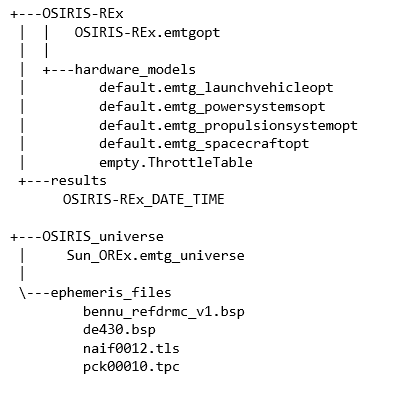
\includegraphics[width=0.6\linewidth]{OSIRIS-REx_folder_structure.png}}
	\caption{\label{fig:folder_structure}Example \ac{EMTG} Mission Directories.}
\end{figure}

%%%%%%%%%%%%%%%%%%%%%
\section{Ephemeris Setup}
\label{sec:ephemeris_setup}
%%%%%%%%%%%%%%%%%%%%%

\ac{EMTG} is most accurate when a \acs{SPICE} kernel is provided for each body of interest but can alternatively use Keplerian orbit elements. Using Keplerian elements will allow \ac{EMTG} to run faster but reduce the accuracy of the solution. In practice, \acs{SPICE} kernels are used most often.

\noindent For this OSIRIS-REx example, all required \acs{SPICE} ephemeris files can be copy/pasted from  \texttt{Tutorial \_EMTG\_Files/OSIRIS\_universe/ephemeris\_files}. Place them in your new \texttt{OSIRIS\_universe/ephe meris\_files}, as shown in Figure \ref{fig:folder_structure}. 

%%%%%%%%%%%%%%%%%%%%%
\subsection{Create Universe File}
\label{sec:create_universe_file}
%%%%%%%%%%%%%%%%%%%%%

An \ac{EMTG} Universe file contains all the body information necessary for a particular Journey of a mission. An \ac{EMTG} Universe file can be created by manually creating a \texttt{.emtg\_universe} text file. For this tutorial, an initial step will be on how to modify an existing Universe text file to include the asteroid Bennu in addition to the planets, Sun, and Moon. The Journey Boundaries and Flybys tutorials will discuss further modification of Universe files. A correctly configured Universe file for all tutorials using the OSIRIS-REx mission is provided in the location: \texttt{Tutorial\_EMTG\_Files/OSIRIS\_universe/Sun\_OREx.emtg\_universe}. This Universe file has the Sun as its central body and the planets, the Moon, and Bennu as secondary bodies.

%%%%%%%%%%%%%%%%%%%%%
\section{Options}
\label{sec:options}
%%%%%%%%%%%%%%%%%%%%%

Now that a sun-centered Universe file with the target asteroid as a body has been created, configure the other mission options by creating and editing an \ac{EMTG} Options file. Open the PyEMTG \ac{GUI} and, in the upper left corner, select File -\textgreater New -\textgreater Mission to open the Mission Options tabs for a new mission. Save this file (Ctrl + s)  as ``OSIRIS-REx.emtgopt'' in the top-level mission directory you created. Tip: Changing the ``Mission Name'' on the ``Global Mission Options'' tab pre-populates the file name in the save-mission dialog. Thus, it is recommended to change the Mission Name, then save the mission. Similarly, it is recommended to always save your \ac{EMTG} options files with the same name as the mission.

%%%%%%%%%%%%%%%%%%%%%
\subsection{Global}
\label{sec:global}
%%%%%%%%%%%%%%%%%%%%%

Select ``Global Mission Options'' if it is not already selected. Then, set the following options as shown in Figure \ref{fig:global_mission_options}:

\begin{itemize}
	\item \textbf{Mission type:} ``\acs{MGAnDSMs}''
	\begin{itemize}
		\item This mission type transcribes chemical maneuvers as impulsive burns along the trajectory and can be used as a low-fidelity model for chemical-propulsion trajectories.
	\end{itemize}
	\item \textbf{Objective function:} ``0: minimum deterministic deltaV''
	\item \textbf{Launch window open date:} ``1 January 2016'' (MJD ``57388.0'')
	\item \textbf{Global flight time bounds(days):} upper bound of ``2256.75'' days
	\item \textbf{Forced post-launch coast duration (days):} ``60'' days
	\begin{itemize}
		\item This is good practice for spacecraft checkout.
	\end{itemize}
	\item \textbf{Forced pre-flyby coast duration (days):} ``45'' days
	\item \textbf{Forced post-flyby coast duration (days):} ``15'' days
	\begin{itemize}
		\item The above forced coast periods for flybys allow for cleanup of trajectory deviations.
	\end{itemize}
\end{itemize}

\begin{figure}[H]
	\centering
	\fbox{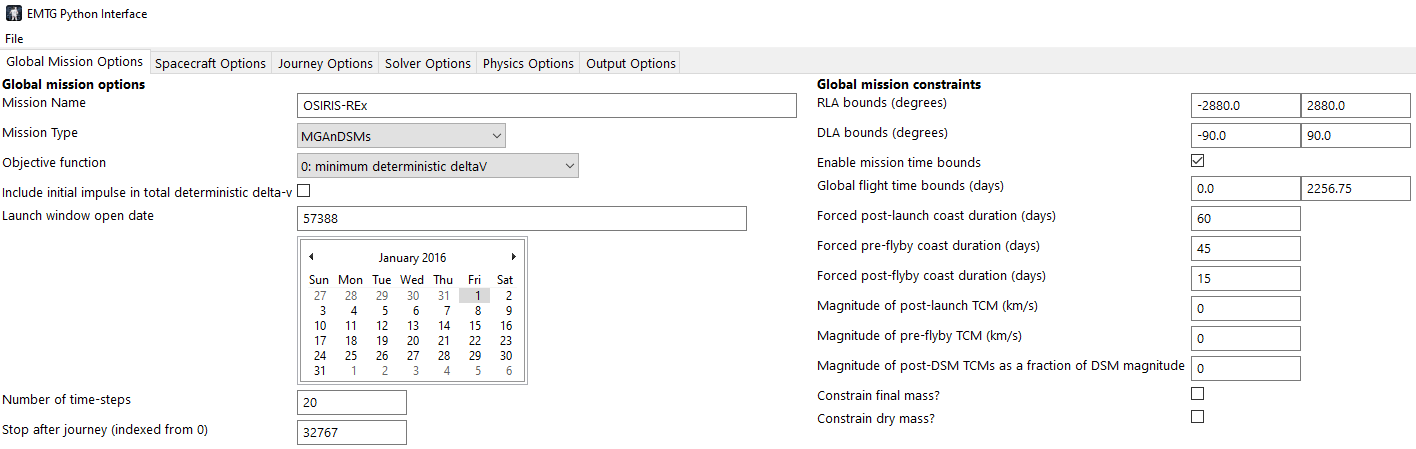
\includegraphics[width=\linewidth]{OSIRIS-REx_global_options.png}}
	\caption{\label{fig:global_mission_options}OSIRIS-REx Global Options.}
\end{figure}

\noindent Try saving the options file again and opening it with a text editor. Opening the options file with a text editor can be done from the \ac{GUI} using the Ctrl + e hotkey. You should see a line with a key-value pair for each of the options that were changed from the default so far.

\noindent \knownissuelabel{Note: There is currently a bug in PyEMTG where if you have assigned a program to open *.emtgopt files, the file will be opened in that program rather than a text editor.}{text_editor_issue} 

%%%%%%%%%%%%%%%%%%%%%
\subsection{Spacecraft}
\label{sec:spacecraft}
%%%%%%%%%%%%%%%%%%%%%

Change to the ``Spacecraft Options'' tab, which sets configuration options for the spacecraft and launch vehicle. Set the following options as shown in Figure \ref{fig:spacecraft_mission_options}:

\begin{itemize}
	\item \textbf{Chemical Isp:} ``230'' seconds
	\item \textbf{Maximum mass:} ``10000'' kg
	\begin{itemize}
		\item  The maximum mass field in this case just scales the optimization problem; the actual launch mass is limited to whatever the launch vehicle can carry to the C3 that the optimizer chooses. (The function relating injected mass to C3 is set in the \ac{EMTG} launch vehicle options file.)
	\end{itemize}
	\item \textbf{Hardware library path:} the path to the \texttt{hardware\_models} directory in the overall mission directory
	\begin{itemize}
		\item Tip: Clicking on the ``...'' button to the left of the input will open a file explorer window where you can select the folder. 
		\item Be sure to include a trailing slash in the path.
	\end{itemize}
	\item \textbf{Launch vehicle library file:} ``default.emtg\_launchvehicleopt''
	\item \textbf{Launch vehicle:} ``ExampleRocket''
\end{itemize}

\begin{figure}[H]
	\centering
	\fbox{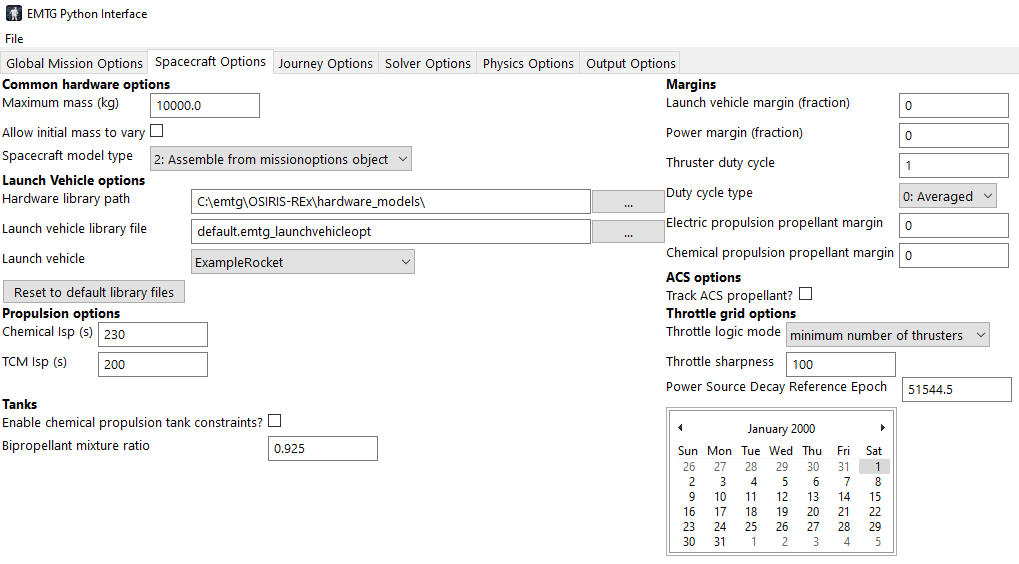
\includegraphics[width=\linewidth]{OSIRIS-REx_spacecraft_options.png}}
	\caption{\label{fig:spacecraft_mission_options}Spacecraft Options.}
\end{figure}

%%%%%%%%%%%%%%%%%%%%%
\subsection{Journey}
\label{sec:journey}
%%%%%%%%%%%%%%%%%%%%%

Select the ``Journey Options'' tab. Each Journey represents a set of events with user-defined boundary conditions. There are many types of Journey departure and arrival conditions; the ones shown here are appropriate for a small body rendezvous. Change the following options on this tab as shown in Figure \ref{fig:earth_to_bennu_journey_options}:

\begin{itemize}
	\item \textbf{Journey name:} ``Earth\_to\_Bennu''
	\item \textbf{Central body:} ``Sun\_OREx.emtg\_universe''
	\begin{itemize}
		\item  Note: If Sun\_OREx does not appear as an option for the central body, the most likely cause is that the default Universe folder was not set to the folder that contains Sun\_OREx.emtg\_universe. To override the default, select the ``Physics Options'' tab, and change the value of the ``Universe folder'' to the folder that contains Sun\_OREx.emtg.universe. Then, return to the ``Journey Options'' tab.
	\end{itemize}
	\item \textbf{Start location:} ``3'' (Earth)
	\item \textbf{Final location:} ``11'' (Bennu)
	\begin{itemize}
		\item These numbers correspond to the integer IDs listed in the Sun\_OREx EMTG Universe file.
	\end{itemize}
	\item \textbf{Wait time bounds (days):} upper bound of ``365.25'' days
	\begin{itemize}
		\item Earth departure can occur up to 365.25 days after the value set for ``Launch window open date'' on the ``Global Mission Options'' tab.
	\end{itemize}
	\item \textbf{Journey inital impulse bounds (km/s):} upper bound of ``5.4102'' km/s
	\item \textbf{Journey arrival type:} ``1: rendezvous (with chemical maneuver)''
	\begin{itemize}
		\item In addition to any DSMs between Earth departure and Bennu arrival, a chemical maneuver will be placed at the final time of the Journey to force the spacecraft to match the position and velocity of Bennu.
	\end{itemize}
	\item \textbf{Flyby sequence:} ``[3]''
	\begin{itemize}
		\item This is a list of Universe body integer IDs. It can have zero, one, or more than one entry. In this case, the list has one element, 3, for Earth because OSIRIS-REx does an Earth flyby on its way to Bennu. Each entry added to the list adds a Phase to the Journey: If a Journey has more than one Phase, they are separated by planetary flybys. In this case, one Earth flyby has been selected, and the Journey has two Phases.
	\end{itemize}
\end{itemize}

\begin{figure}
	\centering
	\fbox{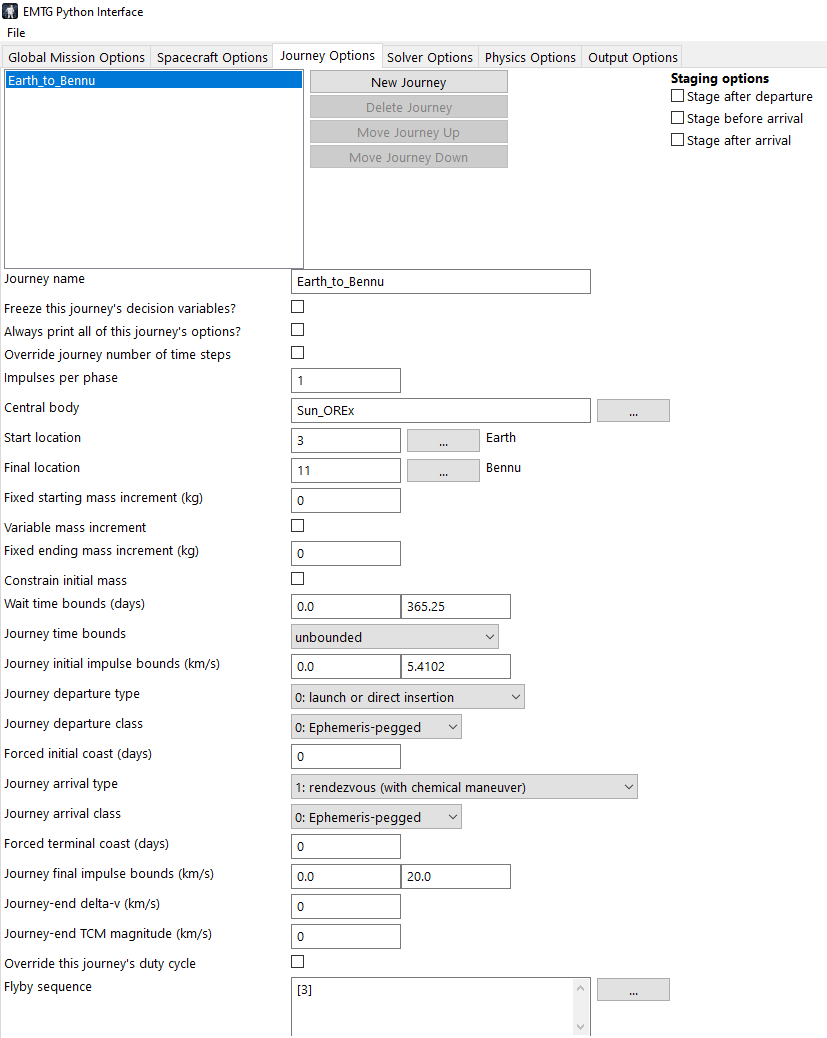
\includegraphics[width=\linewidth]{OSIRIS-REx_earth_to_bennu_journey_options.png}}
	\caption{\label{fig:earth_to_bennu_journey_options}Earth to Bennu Options.}
\end{figure}

\noindent Tip: PyEMTG text boxes can perform basic math operations, so a value of 730.5 can also be achieved by typing ``365.25 * 2'' and deselecting the text input box.

\newpage

\noindent Create a new Journey for the return to Earth by clicking ``New Journey'' and then clicking on ``default'' in the list of Journeys to see the new Journey’s properties. Then, set the following Journey options as shown in Figure \ref{fig:bennu_to_earth_journey_options}:

\begin{itemize}
	\item \textbf{Journey name:} ``Bennu\_to\_Earth''
	\item \textbf{Central body:} ``Sun\_OREx.emtg\_universe''
	\item \textbf{Start location:} ``11'' (Earth)
	\item \textbf{Final location:} ``3'' (Bennu)
	\item \textbf{Wait time bounds(days):} lower bound of ``730.5'' days and upper bound of ``1461.0'' days
	\begin{itemize}
		\item This constrains OSIRIS-REx to spend between 2 and 4 years at Bennu.
	\end{itemize}
	\item \textbf{Journey inital impulse bounds (km/s):} upper bound of ``10'' km/s
	\begin{itemize}
		\item  The initial impulse is an impulsive chemical maneuver applied at the beginning of the Journey. Like the maneuvers at the beginning and end of the ``Earth\_to\_Bennu'' journey, this maneuver does not count against the ``Impulses per phase'' count.
	\end{itemize}
	\item \textbf{Journey arrival type:} ``2: intercept with bounded V\_infinity''
	\begin{itemize}
		\item Here, an Earth arrival as an intercept with bounded v-infinity is being simulated so that the Journey will end with the spacecraft matching the position of the Earth, and the magnitude of the difference between the Earth’s heliocentric velocity and the spacecraft’s heliocentric velocity at this point is constrained. \ac{EMTG} can model the flight path of OSIRIS-REx from the boundary of Earth’s sphere of influence to its interface with the atmosphere and supports a variety of entry constraints. However, this is out of scope for the tutorial. See the scripted constraints document in the \ac{EMTG} repo in \texttt{docs/0\_Users/constraint\_scripting} for more details.
	\end{itemize}
	\item \textbf{Journey final veclocity:} ``6'' km/s
	\begin{itemize}
		\item This is the bound on the V\_infinity of the spacecraft with respect to the arrival body (Earth) at the end of the Journey.
	\end{itemize}
\end{itemize}

\begin{figure}[H]
	\centering
	\fbox{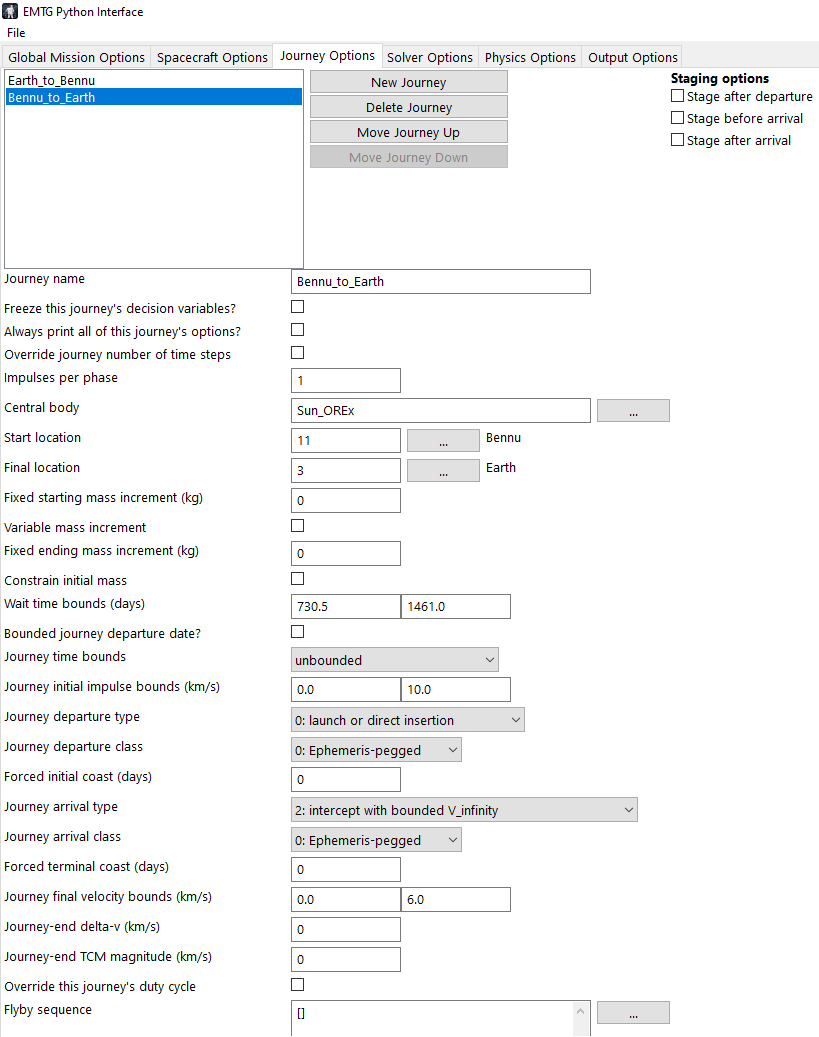
\includegraphics[width=\linewidth]{OSIRIS-REx_bennu_to_earth_journey_options.png}}
	\caption{\label{fig:bennu_to_earth_journey_options}Bennu to Earth Options.}
\end{figure}

%%%%%%%%%%%%%%%%%%%%%
\subsection{Physics}
\label{sec:physics}
%%%%%%%%%%%%%%%%%%%%%

The Physics tab specifies the \acs{SPICE} kernels and configuration to use, force model settings, and state propagation settings. Set the following options as shown in Figure \ref{fig:physics_options}:

\begin{itemize}
	\item \textbf{Universe folder:} the path to the \texttt{OSIRIS-REx/OSIRIS\_Universe} directory
	\item \textbf{Propogator type:} ``Keplerian''
	\begin{itemize}
		\item At this stage of design, ``Keplerian'' is being used because it is much faster than ``Integrator''.
	\end{itemize}
	\item \textbf{Earliest possible SplineEphem epoch:} ``57037.0''
	\item \textbf{Latest possible SplineEphem epoch:} ``60079.0''
	\begin{itemize}
		\item These epoch settings are due to the shortened Bennu ephemeris.
	\end{itemize}
\end{itemize}

\begin{figure}[H]
	\centering
	\fbox{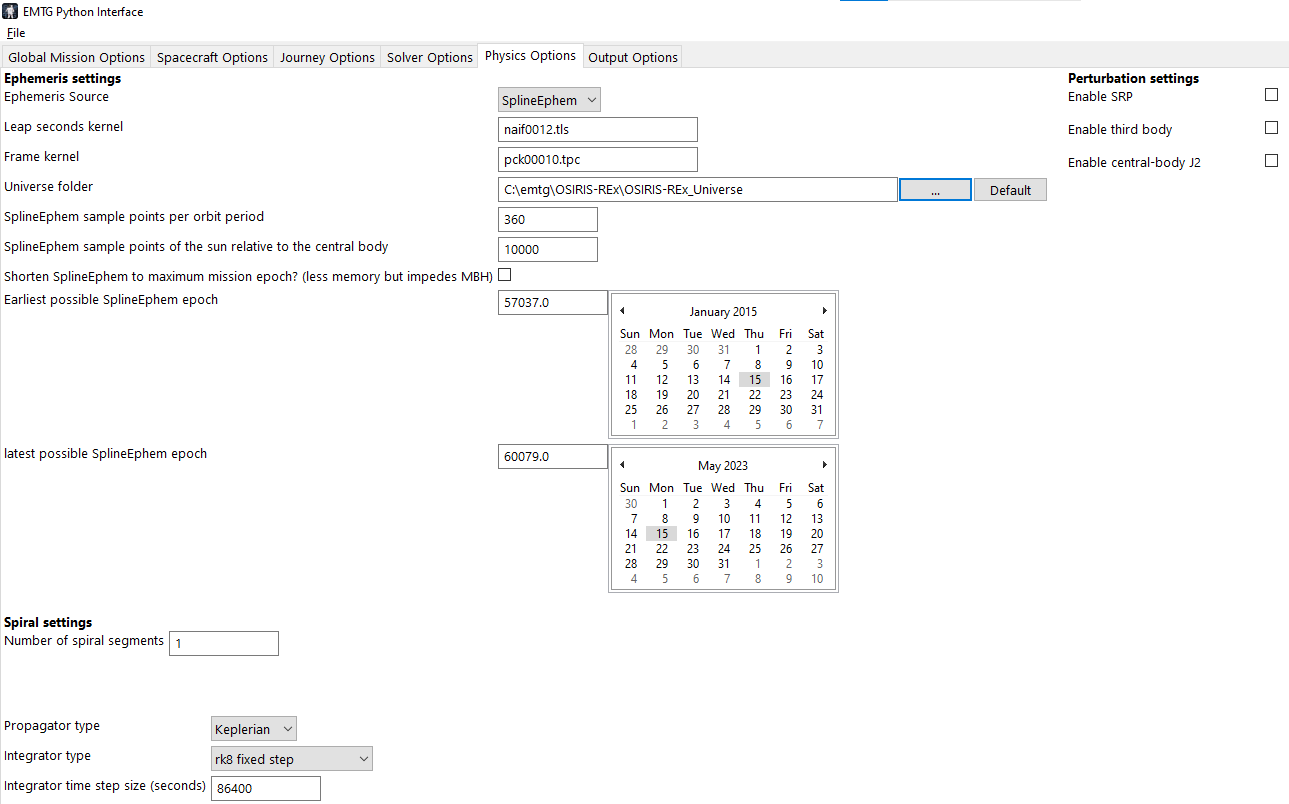
\includegraphics[width=\linewidth]{OSIRIS-REx_physics_options.png}}
	\caption{\label{fig:physics_options}Physics Options.}
\end{figure}

\noindent The ``Perturbation settings'' checkboxes do not work for \ac{MGAnDSMs} Phases with the ``Keplerian'' propagator, so do not check any of them. (Propagation and Phase types will be covered in more detail in later tutorials.)

\begin{figure}[H]
	\centering
	\fbox{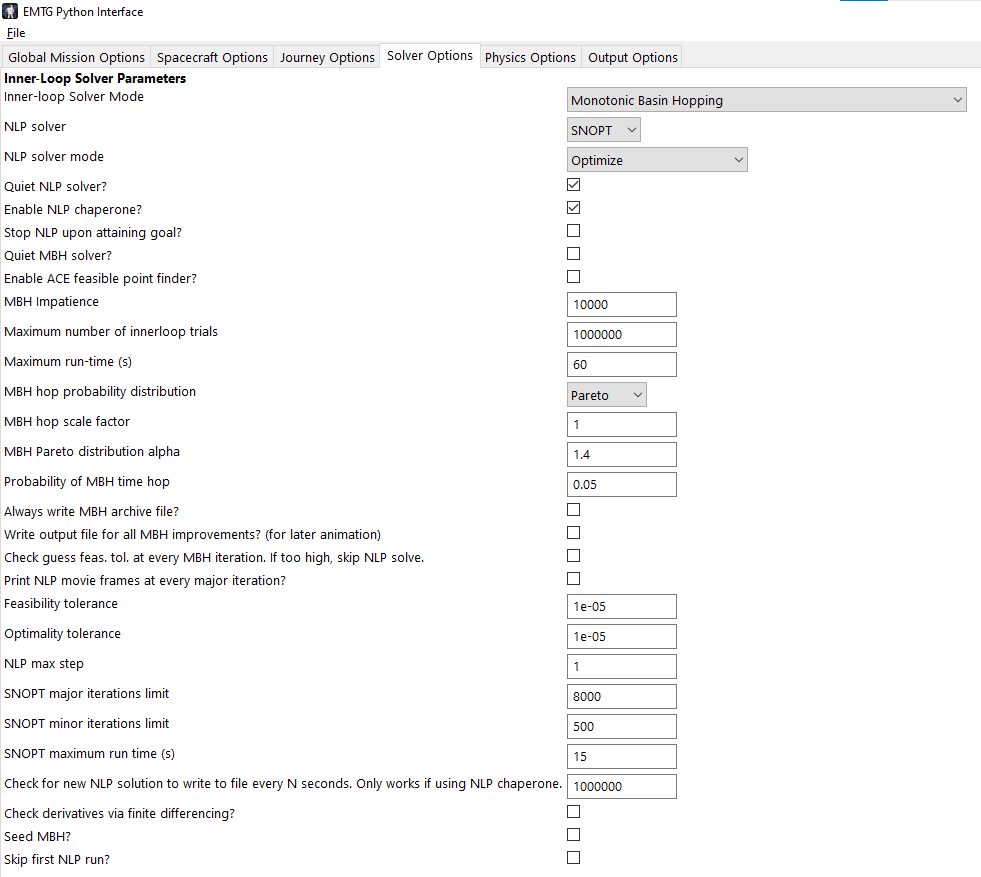
\includegraphics[width=\linewidth]{OSIRIS-REx_solver_options.png}}
	\caption{\label{fig:solver_options}Solver Options.}
\end{figure}

%%%%%%%%%%%%%%%%%%%%%
\subsection{Solver}
\label{sec:solver}
%%%%%%%%%%%%%%%%%%%%%

Switch to the Solver Options tab and set the following options as shown in Figure \ref{fig:solver_options}:

\begin{itemize}
	\item \textbf{Inner-loop Solver Mode:} ``\ac{MBH}''
	\item \textbf{\ac{MBH} hop probability distribution:} ``Pareto''
	\item \textbf{Pareto alpha:} ``1.4''
	\begin{itemize}
		\item For chemical missions like this one, the recommendation is to set the ``Pareto alpha'' to 1.4 (the default) or, if the problem has many local optima, 1.3.
	\end{itemize}
	\item \textbf{ACE feasible point finder:} ``On''
	\begin{itemize}
		\item This settings allows \ac{MBH} to compare infeasible solutions and search for minimum infeasibility before it finds its first feasible solution and begins to search for optimality. In most cases, it is recommended to have the ACE feasible point finder on.
	\end{itemize}
	\item \textbf{\ac{NLP} chaperone:} ``On''
	\begin{itemize}
		\item This settings enables \ac{EMTG} to recover the best solution found in a run of \ac{SNOPT} even if \ac{SNOPT} does not converge. In most cases, it is recommended to have the \ac{NLP} chaperone on.
	\end{itemize}
\end{itemize}

%%%%%%%%%%%%%%%%%%%%%
\subsection{Output}
\label{sec:output}
%%%%%%%%%%%%%%%%%%%%%

\noindent Switch to the Output Options tab and set the following options as shown in Figure \ref{fig:output_options}:

\begin{itemize}
	\item \textbf{Background mode:} ``Off''
	\begin{itemize}
		\item Background mode means ``close \ac{EMTG} as soon as it is done executing''. If you are running \ac{EMTG} from PyEMTG, then you should leave background mode off so that you can see your results more easily.
	\end{itemize}
	\item \textbf{Print only non-default options to .emtgopt file:} ``On''
	\begin{itemize}
		\item This settings means write a short-form emtgopt file that takes up less space on your hard drive. Options that have their default value are not written to the file. If this option is unchecked, all options are written to the emtgopt file, regardless of whether or not they have their default value.
	\end{itemize}
	\item \textbf{Output file frame:} ``\acs{ICRF}''
	\item \textbf{Override working directory:} ``On''
	\item \textbf{Working directory:} create the \texttt{OSIRIS-REx/results} directory and set this to the path to that directory
	\begin{itemize}
		\item This will cause \ac{EMTG} to place its results in this folder instead of the default location inside the \ac{EMTG} repo, and lets you keep the results with the \ac{EMTG} options files that created them.
	\end{itemize}
\end{itemize}

\begin{figure}[H]
	\centering
	\fbox{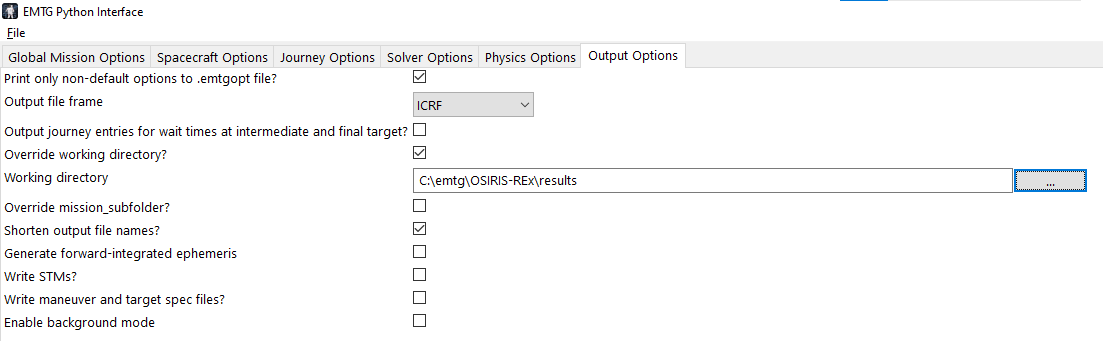
\includegraphics[width=\linewidth]{OSIRIS-REx_output_options.png}}
	\caption{\label{fig:output_options}Output Options.}
\end{figure}

%%%%%%%%%%%%%%%%%%%%%
\section{Run Mission}
\label{sec:run_mission}
%%%%%%%%%%%%%%%%%%%%%

Select File-\textgreater Run as shown in Figure \ref{fig:running_mission}. PyEMTG will prompt you to save an emtgopt options file to ensure that your emtgopt file is saved to disk prior to executing \ac{EMTG}. (The same prompt as if you selected File-\textgreater Save.) \ac{EMTG} will then execute, create a new timestamped subdirectory for your results within your results directory, and begin solving your problem. You can also save and run the mission from the command line by passing the emtgopt file as a command-line argument to the executable. For example, replacing ``\textless EMTG-FOLDER\textgreater '' and ``\textless OSIRIS-REx\textgreater '' folder with the correct paths and running: \newline \texttt{C:\textbackslash<EMTG-FOLDER>\textbackslash bin\textbackslash EMTGv9.exe C:\textbackslash<OSIRIS-REx-FOLDER>\textbackslash OSIRIS-REx.emtgopt}

\begin{figure}[H]
	\centering
	\fbox{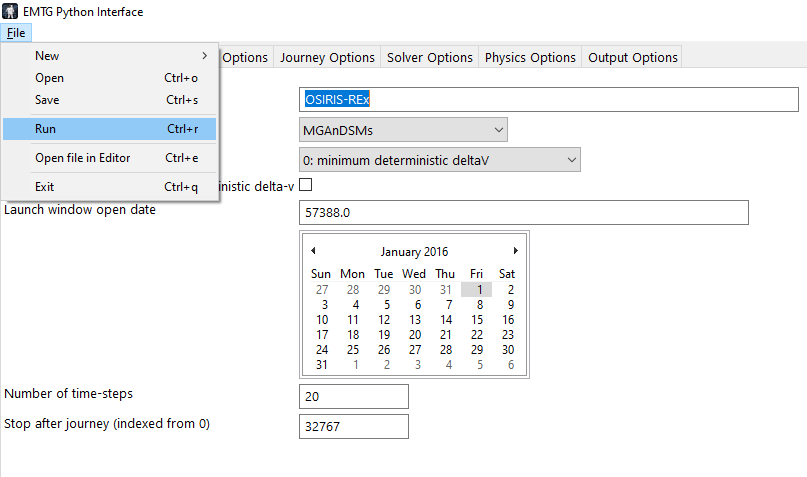
\includegraphics[width=0.9\linewidth]{OSIRIS-REx_run_mission.png}}
	\caption{\label{fig:running_mission}Running a mission.}
\end{figure}

\noindent While running, \ac{EMTG} outputs information about its progress to the command window in which it is executing, showing information about the current decision vector feasibility and optimality compared to the best solution found so far. Since the Bennu \acs{SPICE} kernel used covers a smaller range of time than DE430, you may see occasional \acs{SPICE} errors, but the run should still finish. (Even if a given \ac{SNOPT} run fails, the next \ac{MBH} iteration will start normally.) If everything is configured correctly, you should see output similar to Figure \ref{fig:example_output} when the \ac{EMTG} run ends. (The \ac{EMTG} run will last about 1 minute; this can be configured in the ``Solver Options'' tab.) Note that, due to the short run time used for \ac{EMTG} and the stochastic nature of \ac{MBH}, your ``Best value found'' may not be the same as that shown in Figure \ref{fig:example_output}, but it is very likely that \ac{EMTG} will at least find a feasible solution. Your results subdirectory will contain, among other files, a .emtg file that describes the solution.

\begin{figure}[H]
	\centering
	\fbox{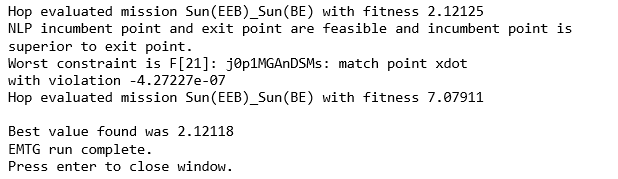
\includegraphics[width=0.9\linewidth]{OSIRIS-REx_example_output.png}}
	\caption{\label{fig:example_output}Example \ac{EMTG} run output.}
\end{figure}

%%%%%%%%%%%%%%%%%%%%%
\section{Post-Process}
\label{sec:rpost_process}
%%%%%%%%%%%%%%%%%%%%%

The .emtg solution file contains the final trajectory, objective value, scaling information, Journey events, and other information to describe the trajectory. It can also be used as an initial guess for other \ac{EMTG} runs. This feature is covered in other tutorials. For now, open the .emtg file in the results directory in a text editor and look through the information contained inside. An example file is shown in Figure \ref{fig:emtg_output_file}.

\begin{figure}[H]
	\centering
	\fbox{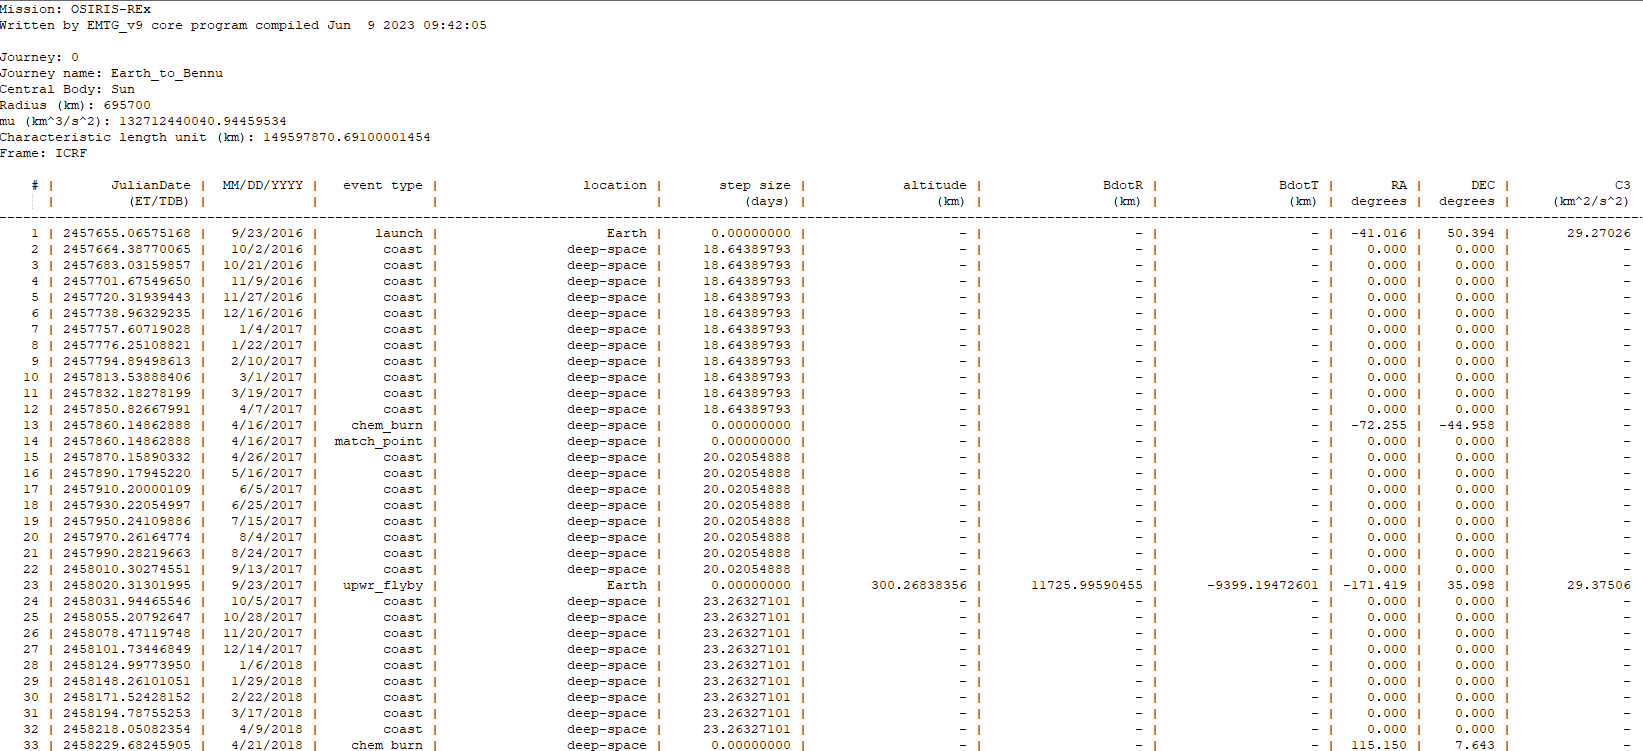
\includegraphics[width=\linewidth]{OSIRIS-REx_EMTG_output_file.png}}
	\caption{\label{fig:emtg_output_file}Selection from .emtg solution file.}
\end{figure}

\noindent PyEMTG can open .emtg files as shown in Figure \ref{fig:PyEMTG_opening_emtg_file}. PyEMTG can create basic trajectory plots and systems summary plots, and process various other \ac{EMTG} outputs. For this example, the trajectory plot will be focused on. PyEMTG can also search for targets of opportunity along your trajectory. This is out of scope for the tutorial.

\begin{figure}[H]
	\centering
	\fbox{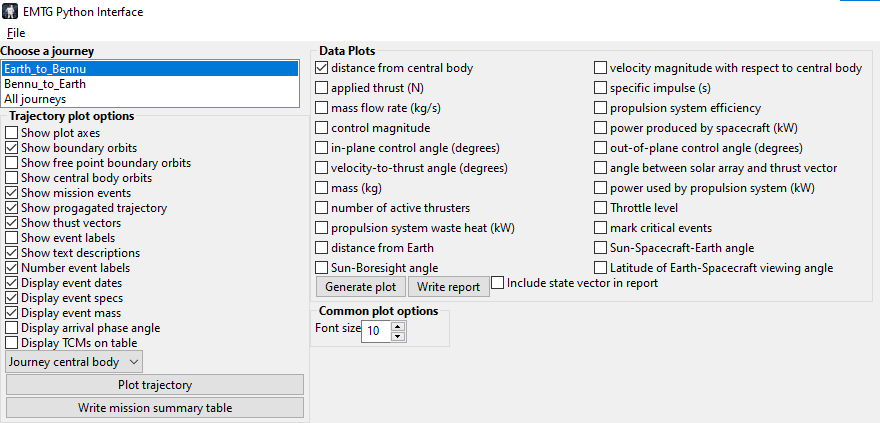
\includegraphics[width=\linewidth]{OSIRIS-REx_opening_EMTG_file.png}}
	\caption{\label{fig:PyEMTG_opening_emtg_file}A .emtg file in PyEMTG.}
\end{figure}

\noindent Open the .emtg file in PyEMTG by selecting File-\textgreater Open and navigating to the file. Try plotting the results by selecting ``All journeys'' and ``Show event labels'', then clicking ``Plot trajectory''. You should see something similar to Figure \ref{fig:traj_plot}. Note that PyEMTG’s plotting utilities are quite basic. For more advanced plotting, the workflow is to use an \ac{EMTG} solution to create a bsp and import the bsp into a tool like \ac{GMAT} or \ac{STK}. Using an \ac{EMTG} solution to create a bsp is beyond the scope of this tutorial.

\begin{figure}[H]
	\centering
	\fbox{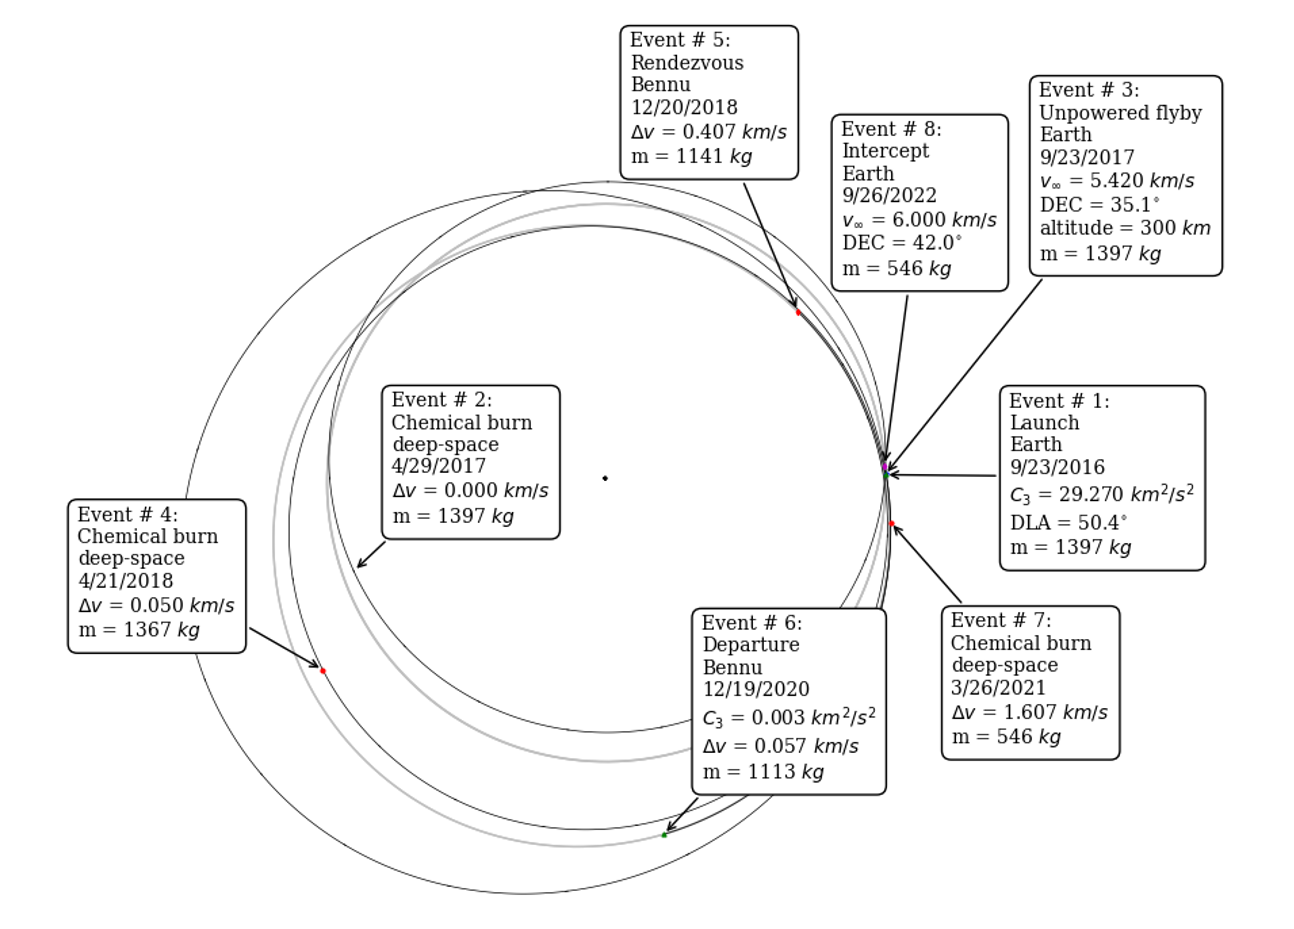
\includegraphics[width=\linewidth]{OSIRIS-REx_trajectory_plot.png}}
	\caption{\label{fig:traj_plot}Example \ac{EMTG} trajectory plot.}
\end{figure}

\noindent This concludes the first \ac{EMTG} tutorial! This mission is the basis for the low-thrust OSIRIS-REx tutorial, LowSIRIS-REx.


\end{document}